The proposed pipeline, described in Fig.~\ref{fig:pipeline}, provides the steps undertaken to perform the desired packing. The baseline steps correspond to: 
\begin{myitem}
\item[a)] {\em (Sensing)}: sense and select a target object $o^i$ to pick up;
\item[b)] {\em (Picking)}: execute action $\{\tt pick\}$; 
\item[c)] {\em (Transfer)}: move $o^i$ to the next available target pose $\hat{p}^j$ and execute action $\{\tt release\}$.
\end{myitem}
The experimental section considers this baseline pipeline, where it is observed that it performs poorly due to multiple sources of uncertainty, ranging from pose estimation and calibration errors, to object non-uniformity and object interaction with the bin and other objects, among others. These issue necessitate the introduction of remedies, which actively reduce the impact of the uncertainty. To this end, 3 manipulation primitives for a simplistic end-effector are designed to increase robustness and are integrated with the overall architecture: 
\begin{myitem}
\item[i)] Toppling;
\item[ii)] Robust Placement; and 
\item[iii)] Corrective Packing.
\end{myitem}

%\subsection{Baseline - Without Pose Estimation}
%A placement module informs the task planner of the position and orientation of the dropped objects.After an object is picked up, the robot will directly move to the target position and drop the object. 

%\subsection{Packing While Trusting Pose Estimation}
%For different objects, the transform between the grasped object and the end-effector is different, given the target pose of the object, adjustments of the pose of the grasped object can be done to attempt to align it to the desired drop positions.

\subsection{Baseline: Pose Estimation and Picking}
Given an RGB-D image of the source bin and a CAD model of the object, the objective is to retrieve ($\object^i$, $\pose^i$) such that it maximizes the chance of achieving target configuration $\hat{p}^j$, where $D(p^i,\hat{p}^j) \leq \epsilon$. To achieve this, the image is passed through a {\tt MaskRCNN} convolutional neural network~\cite{he2017mask}, which is trained to perform segmentation and retrieve the set of object instances $\objectset$.  An image segment is ignored if it has a number of pixels below a threshold. It is also ignored, if {\tt MaskRCNN} has small confidence that the segment corresponds to the target object. Among the remaining segments, instances $\object^i \in \objectset$ are arranged in a descending order of the mean global Z-coordinate of all the RGBD pixels in the corresponding segment. Then, 6D pose estimation is performed for the selected instance~\cite{175}\cite{stocs}. 

If, given the detected 6D pose of the instance, the top-facing surface does not allow the placement of the object via a top-down pick, the next segment instance is evaluated in order of the mean global Z-coordinate. If no object reveals a top-facing surface, then the first object in terms of the maximum mean global Z-coordinate is chosen for picking. 

For the selected object, a picking point, i.e., a point where the suction cup will be attached to the object, is computed over the set of points registered against the object model. It utilizes a picking-score associated in a pre-processing step with each model point, which indicates the stability of the pick on the object's surface. The score calculates the distance to the center of the object mesh. A continuous neighborhood of planar pickable points is required to make proper contact between the suction cup and the object surface. Thus, a local search is performed around the best pick-score point to maximize the pickable surface.


% For the arm to pick $\object^i$ at $\pose^i$, it has to be that the arm's end-effector pose satisfies certain conditions relative to the object's pose as expressed by a binary output function: $\mathtt{is\_pick\_feasible}( \object^i, \pose^i, \grasp), \textrm{ where } \grasp \in \mathcal{T}.$ For instance, the pose $\grasp$ of a suction cup must align it with at least one of the surfaces of an object $\object^i$ at $\pose^i$. Then, it is possible to define the set of end-effector poses, which allow to pick an object at a specific pose: \vspace{-.05in}$$\graspset( \object^i, \pose^i ) = \{\grasp \in \mathcal{T}:  {\mathtt{is\_pick\_feasible}}(\object^i, \pose^i, \grasp) = true\}. \vspace{-.05in}$$ 

% Assume the sets $\graspset( \object_i, \pose_i )$

\subsection{Toppling}
% \commentadd{
% An error in the picking action or the absence of objects exposing top-facing surfaces allowing placement of the object with a single pick, necessitates a strategy to expose a desired pickable surface of the object.
% }
\rahul{
% \begin{figure}
%     \centering
%     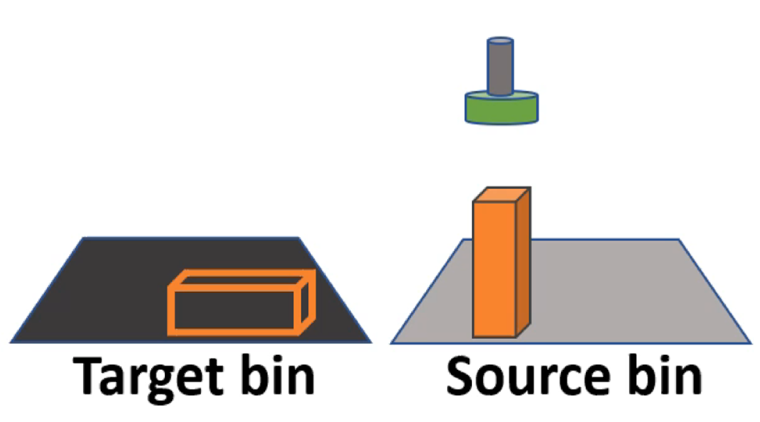
\includegraphics[width=0.3\textwidth]{Figures/toppling_begin.png}
%     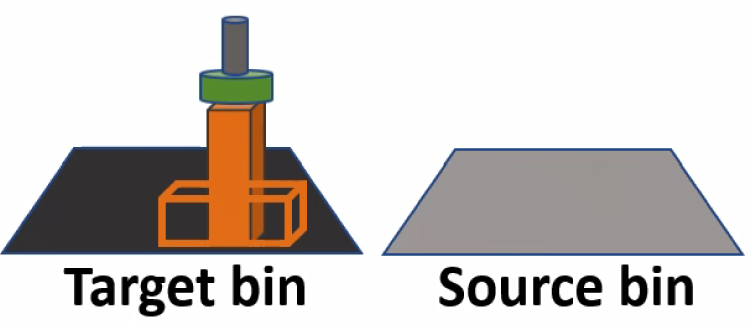
\includegraphics[width=0.3\textwidth]{Figures/toppling_end.png}
%     \caption{An illustration of a scene where a direct pick-and-place fails to solve the problem without reorienting the object. The \textit{top} image shows the initial scene where the orange cuboidal object needs to be transferred to the target bin at the pose denoted by the wireframe marker. The \textit{bottom} image shows the end-effector placing it using a top-down grasp.}
%     \label{fig:reorientation_failure}
% \end{figure}
}
The toppling primitive is invoked if there exists no object that exposes the desirable top-facing surface, or if the object was erroneously picked from the wrong face. The latter is detected after the pick by performing pose estimation once the objet is attached to the suction cup. For instance this can happen for the soaps shown in Figure \ref{fig:pipeline} (right)(d), if the thin side is available for pick but the soap needs to be placed on their wider side. In this case, a toppling primitive is used to reorient the object.
\rahul{
% \begin{figure*}
%     \centering
%     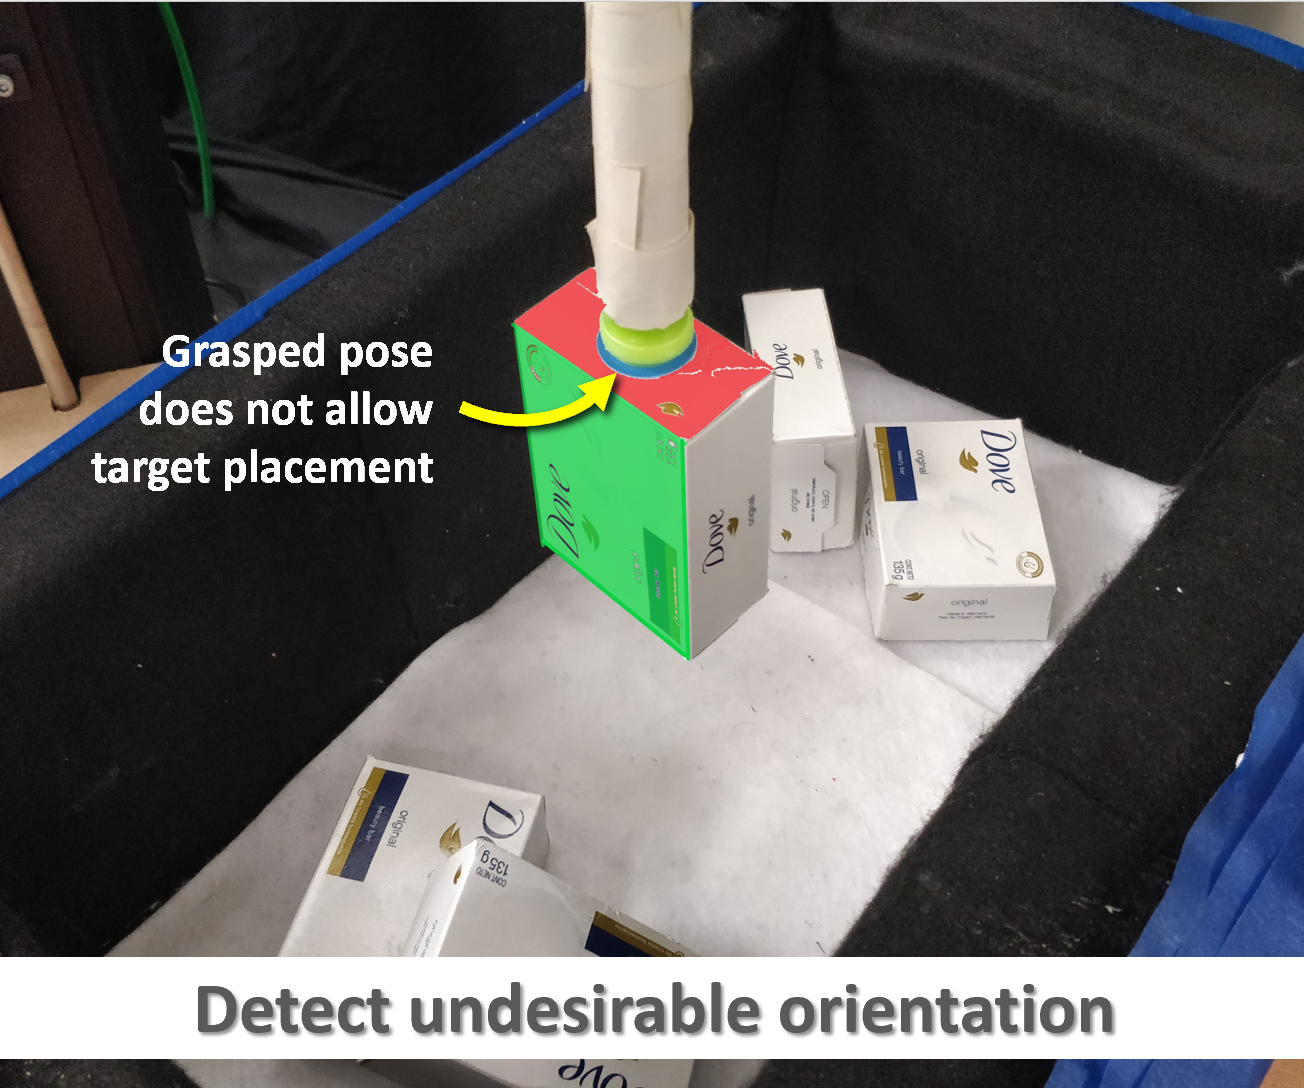
\includegraphics[width=0.24\textwidth]{Figures/toppling1.png}
%     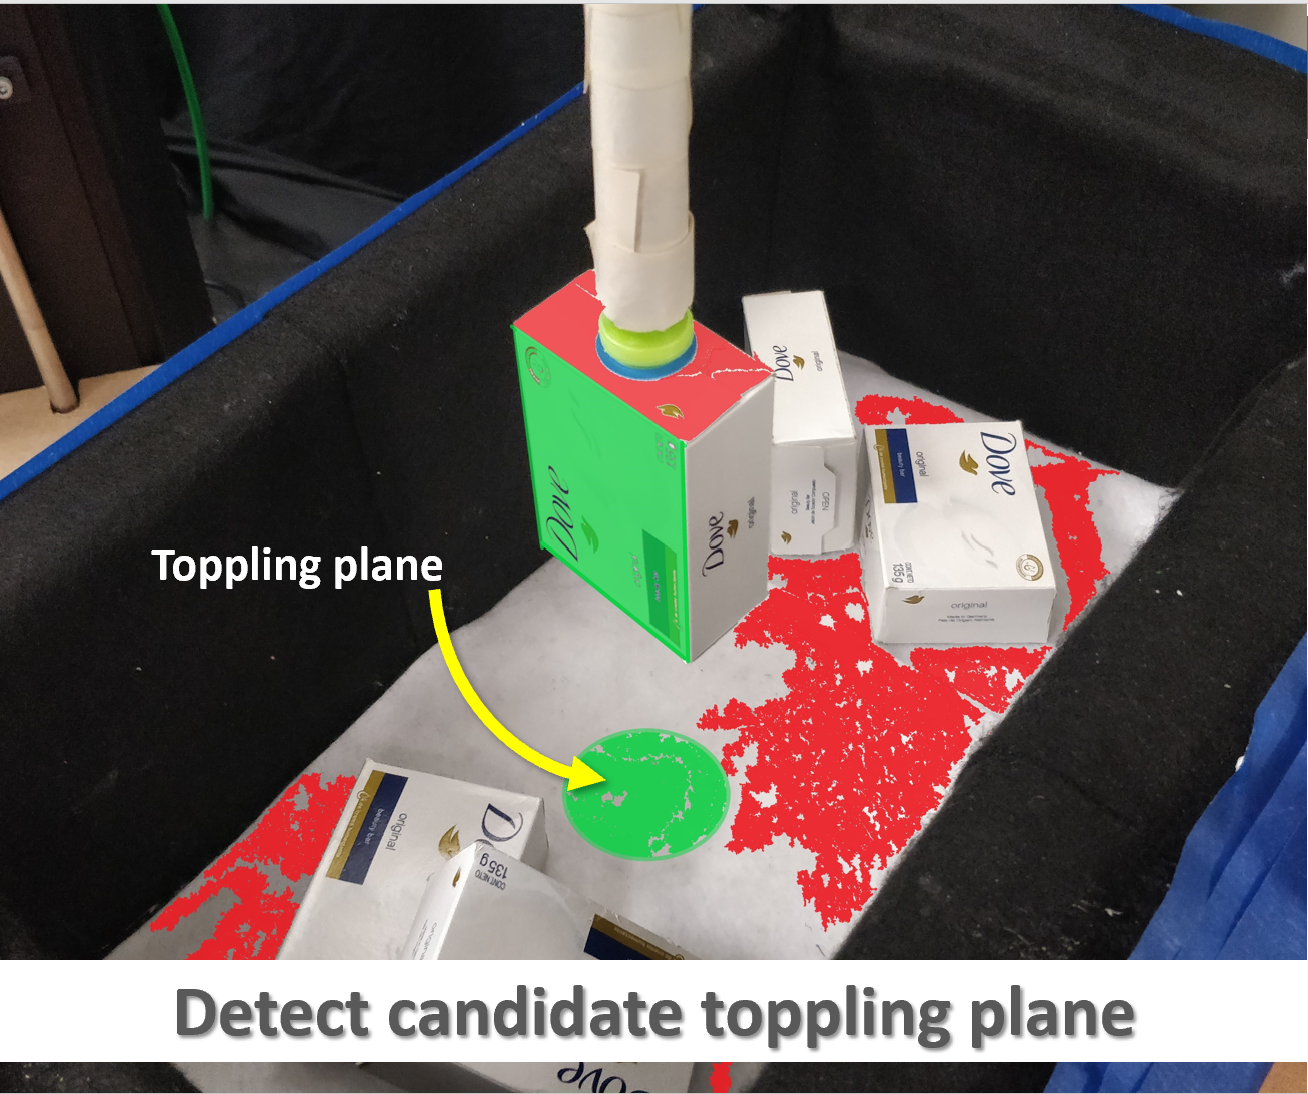
\includegraphics[width=0.24\textwidth]{Figures/toppling2.png}
%     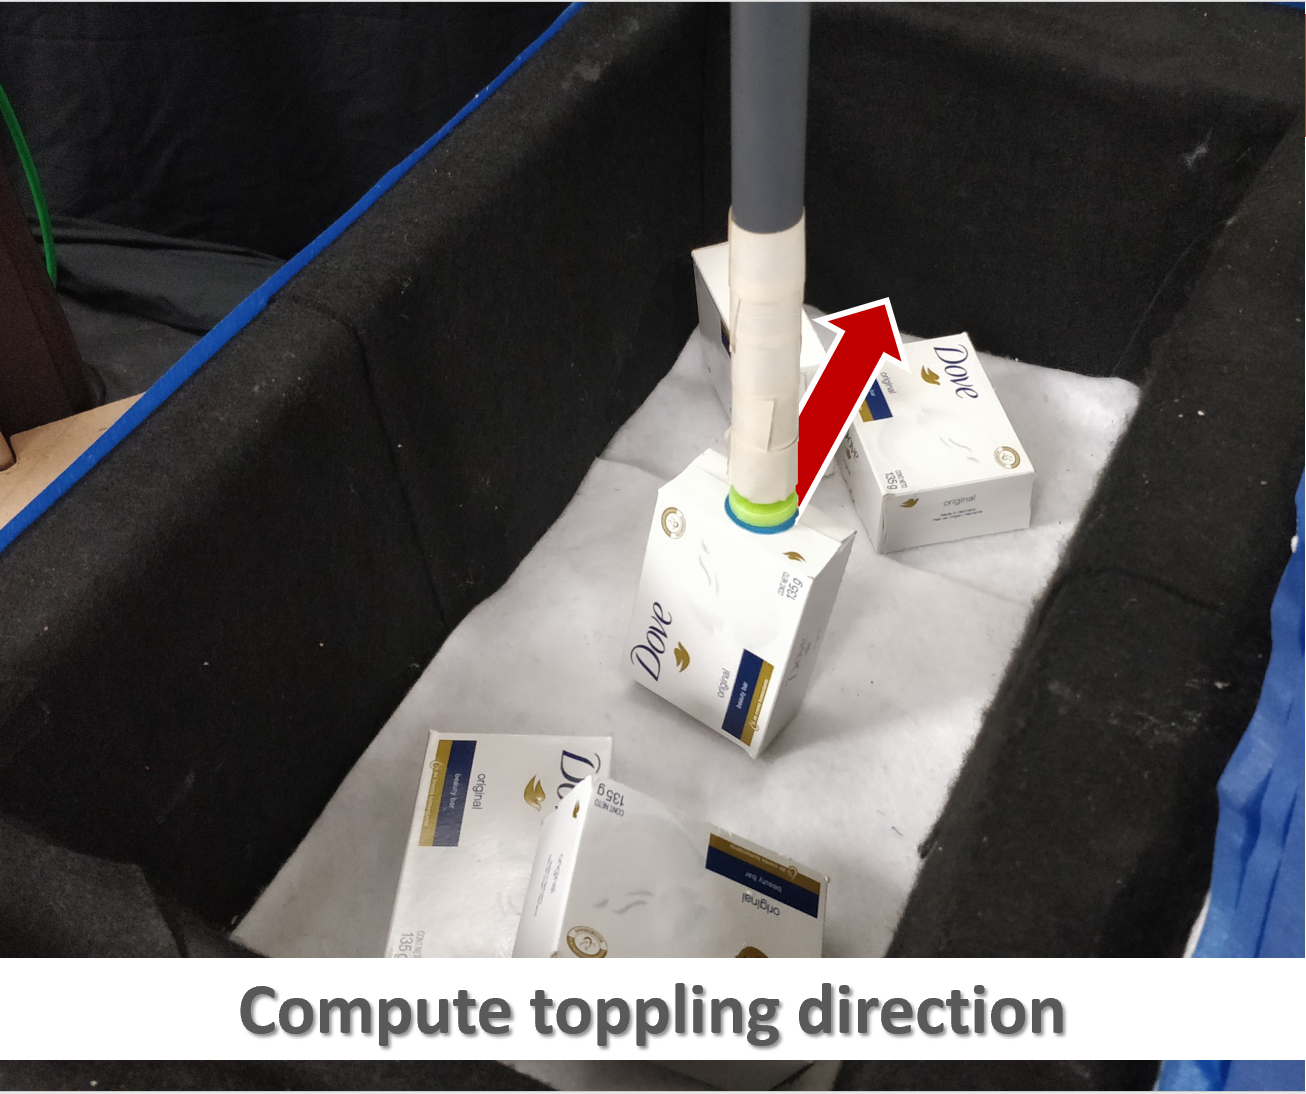
\includegraphics[width=0.24\textwidth]{Figures/toppling3.png}
%     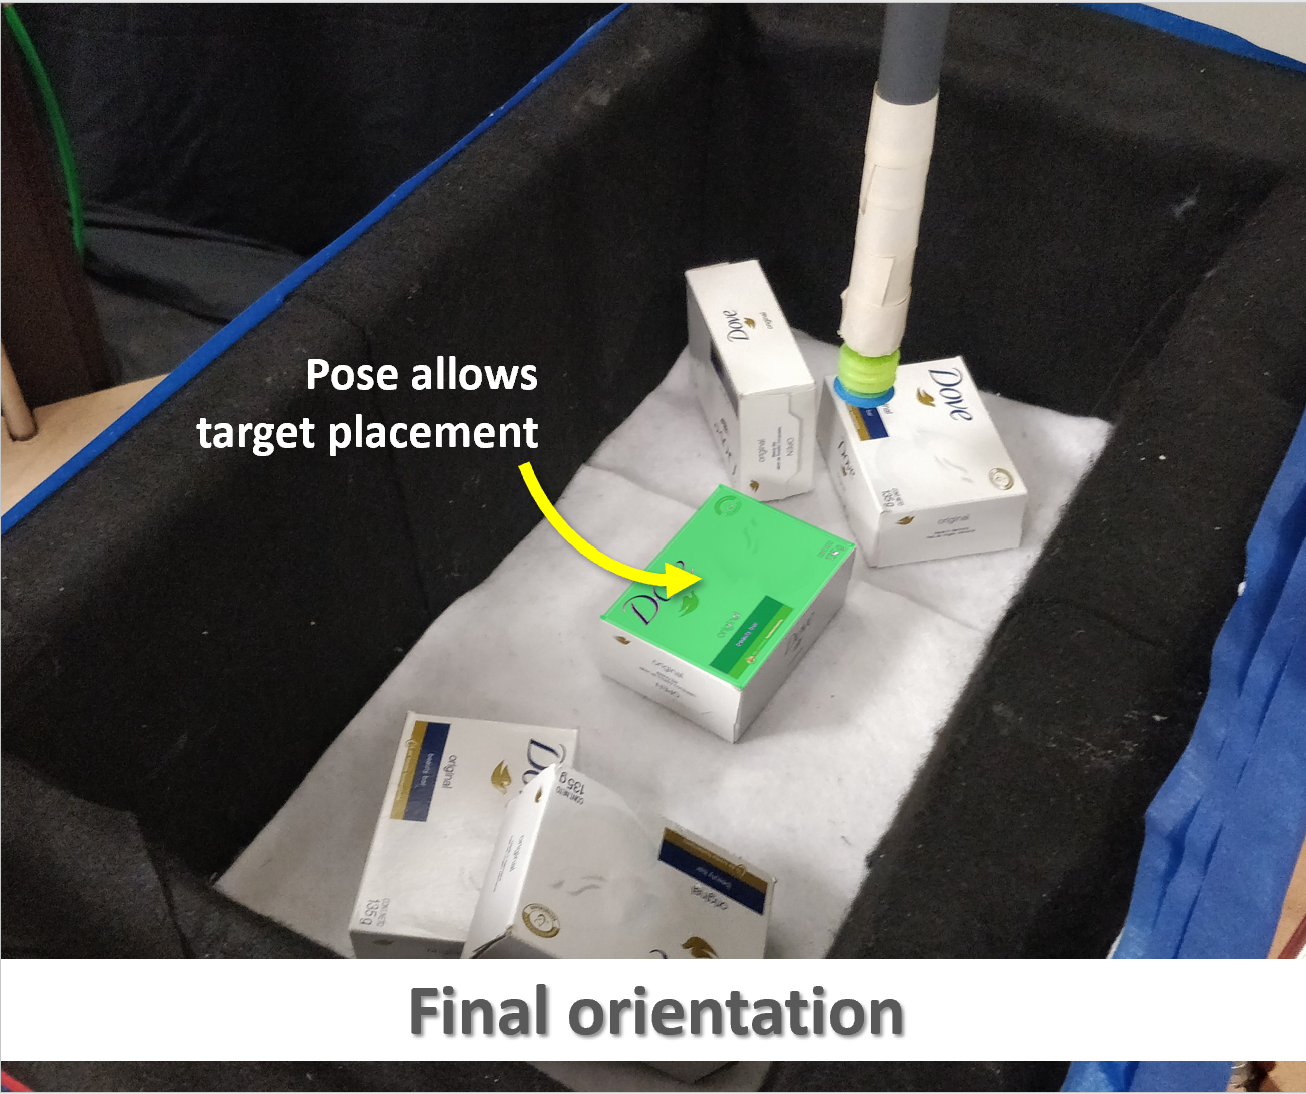
\includegraphics[width=0.24\textwidth]{Figures/toppling4.png}
%     \caption{Steps of toppling primitive from left to right. \textit{Firstly,} the scenario where the grasped pose of the object does not allow the target placement is detected, \textit{secondly,} a plane is detected in the scene that can allow toppling, \textit{thirdly,} the toppling direction is computed and executed, and \textit{finally,} the reoriented object rests in a pose that allows the target placement.}
%     \label{fig:toppling_steps}
% \end{figure*}

\begin{figure*}
    \centering
    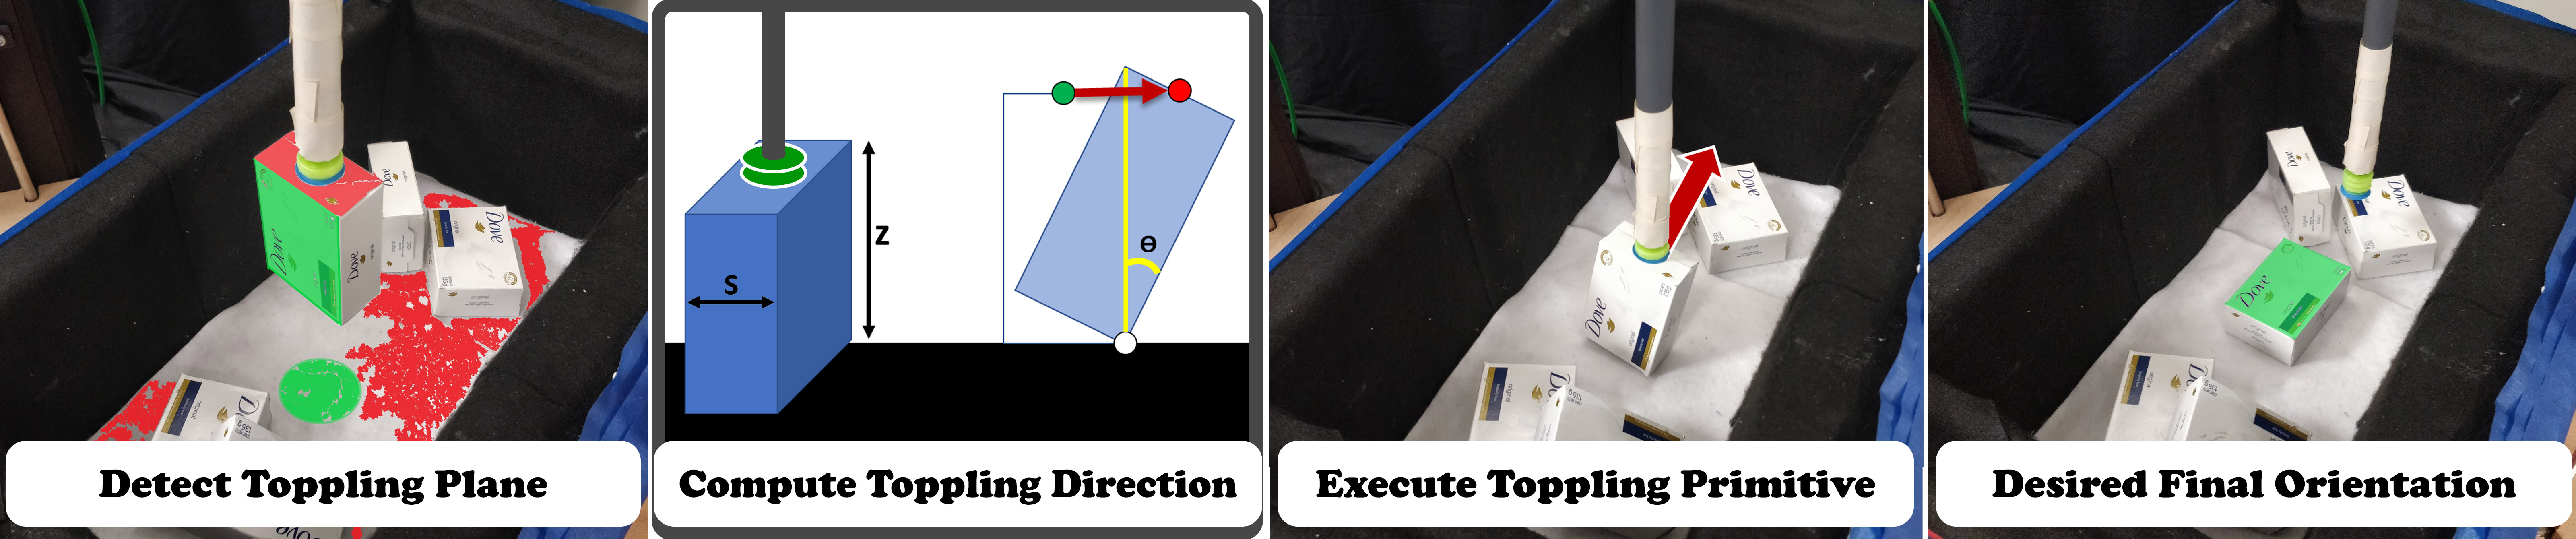
\includegraphics[width=1\textwidth]{Figures/toppling}
    \caption{Steps of toppling primitive from left to right when the scenario where the grasped pose of the object does not allow the target placement is detected. \textit{Firstly,} a plane is detected in the scene that can allow toppling, \textit{secondly,} the toppling direction is computed and \textit{thirdly} executed, and \textit{finally,} the reoriented object rests in a pose that allows the target placement.
    An illustration showing the toppling vector computation with (a) shows the dimensions of the object with \textit{s} being the dimensions along the side that exposes a desired face, and \textit{z} being the height of the top face. On the right, (b) shows the topping vector under the assumption that the object was grasped from the center of the face.
    }
    \label{fig:toppling_steps}
\end{figure*}
}

% The candidate object $o^i$ should be transferred if its detected pose $\pose_{start}$ allows, when moved to $\btarget$, to the next available target pose $\hat{p}^j$. But it could be that while $\graspset( \object^i, \pose_{start} ) \neq \emptyset$, the pose $\pose_{start}$ does not allow the arm to move the object to the target bin in a way that to achieve $\hat{p}^j$. 
% }
% For instance this can happen for the soaps shown in Figure \ref{fig:pipeline} (right), if the thin side is available for pick but the soap needs to be placed on their wider side. 
% In this case, a toppling primitive is used to reorient the object. The toppling primitive is invoked if there exists no object that exposes the desirable picking surface, or if the object was erroneously picked from the wrong face, which is detected after the pick by performing pose estimation on it. 
%Taking into account reachability, collisions and limited symmetry relaxations $\mathbb{P}_{INV}$ can be significantly large enough. A packing method cannot be complete unless there is some explicit reasoning about this set of poses.
%Within the classes of available actions $\{ \mathtt{pick}, \mathtt{release} \}$ a fixed attachment is enforced during a $\mathtt{pick}$, and the constraint is removed during a $\mathtt{release}$. 
% \commentadd{
% Given a starting pose of an object $\pose_{start}$, let the operation $\pose_{topple} = \mathbb{TR}(\pose_{start}, \Pi_{start} )$ represent the pose of the object at the end of the set of actions $\Pi_{topple}: [0,1] \rightarrow \mathcal{X}$ of the arm, defined in the full state space. A toppling action sequence $\Pi_{topple}$ attempts to find a sequence of motions that bring the pose of the object $o^i$ to $\pose_{topple} = \mathbb{TR}(\pose^i, \Pi_{topple} )$, so that:
% % \vspace*{-5mm}
% \begin{equation}
% \exists\ \Pi_{transfer}, \textrm{ so that } D( \mathbb{TR}( \pose_{topple}, \Pi_{transfer} ), \hat{p}^j)  \leq \epsilon
% \label{eq:topple}
% \end{equation}
% }

Given a starting pose of an object $\pose_{start}$ and a toppling action of the arm, the object ends up at a new pose $\pose_{topple}$. The objective is to allow the existence of a pick $\hat{g} \in \graspset( \object^i, \pose_{topple} ) $ so that there is a $\mathtt{transfer}$ action from pick $\hat{g}$ that achieves the final  placement $p_{end}$ close enough to the desired target placement $\hat{p}^j$, i.e., $D(p_{end},\hat{p}^j) \leq \epsilon$. For the considered setup, this means that the top-facing surface of the object at $\pose_{topple}$ and $\hat{p}^j$ is the same.

The toppling module inspects the visible point cloud in the source bin to identify the best toppling plane, which is sufficiently empty and flat. The accompanying implementation restricts actions to ones that change the pose of the cubic objects by shifting the most upward facing surface to only one of the adjacent surfaces. While this does not guarantee toppling the object to all possible poses, the symmetry of cubic products resolves this issue. 

Prior work \cite{lynch1999toppling} has shown the efficacy of minimal end-effectors used in tandem with the environment to achieve toppling. In the previous work, the friction against a conveyor belt is used to topple an object about a resting surface. The conveyor belt's motion is parallel to the initial resting surface plane. In the current setup, the compliance of the suction cup is used to emulate the same effect using a lateral motion on the same plane as the top-surface along the direction of the desired transformation between $\pose_{start}$ and $\pose_{topple}$. Due to symmetry, at least one neighboring surface allows top-down picks, so a successful toppling action exists. Using the pose of the object, the lateral motion direction is executed once the object is placed on the detected plane, and the object is released during this action. Results show that this is highly effective in the target setup.

% of satisfying Eq. \ref{eq:topple}. 

% A high level subroutine in the context of the pipeline is demonstrated as follows.



\rahul{
% \begin{figure}[t]
%     \centering
%     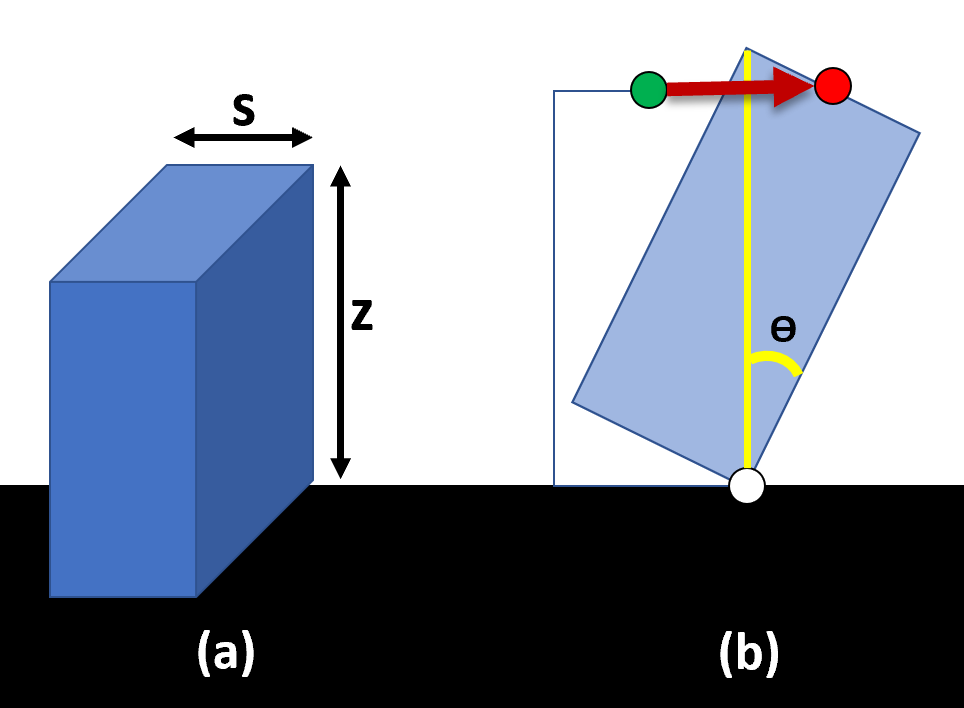
\includegraphics[width=0.48\textwidth]{Figures/toppling_direction.png}
%     \caption{An illustration showing the toppling vector computation with (a) shows the dimensions of the object with \textit{s} being the dimensions along the side that exposes a desired face, and \textit{z} being the height of the top face. On the right, (b) shows the topping vector under the assumption that the object was grasped from the center of the face.}
%     \label{fig:toppling_direction}
% \end{figure}

Algorithm~\ref{algo:topple} describes the high-level sequence of steps involved in executing a toppling action. This subroutine will be invoked once the object is already attached to the end-effector using a top-down grasp, and is also visible to the camera in order to obtain a point cloud. It returns a sequences of poses that constitute the discrete steps of the toppling maneuver, which when executed should drop the object to expose a desired face, denoted by the target orientation.
Line 2 checks whether such a reorientation is even necessary by using the symmetry aware distance between the current grasped pose, and the desired pose. The toppling plane is obtained by estimating a large enough (based on the dimensions of the bottom surface of the object) planar surface on the point cloud, that is also priorized to prefer lower planes than expectedly more unstable higher surfaces on the pile. 

The {\tt GetOffset} primitive is described in Fig~\ref{fig:toppling_steps} (second) to show the computation of the toppling maneuver. Given the pose of the object, the height of the top face is denoted by \textit{z}. Given the desired face(s) that needs to be exposed as the top face to allow the target placement using a top-down grasp, \textit{s} denotes the dimension of the edge(s) not adjacent to the desired face; i.e., out of the two dimensions defining the top-face, select the one that corresponds to the direction of toppling. Define $\theta = \tan^{-1} \frac{s}{z} $. The toppling has to change the orientation of the object till its center (approximating the center of gravity) goes beyond the support point at along the contact edge denoted by the white circle in the image. This object rotation can be affected by displacing the grasp point of contact (green circle) to the {toppled configuration} (red circle). Without loss of generality, consider the point of grasp to be the center of the top face. The offsets become:

\vspace{-0.2in}
$$
	\Delta x = \frac{s}{2} + z \sin \theta - \frac{s}{2} \cos \theta + \epsilon;\ 
	\Delta z = z \cos \theta + \frac{s}{2} \sin \theta - z
$$
\vspace{-0.15in}

Here $\Delta x$ and $\Delta z$ denote the planar and height offsets in the object's local frame describing the toppling vector, shown by the red arrow in Fig~\ref{fig:toppling_steps} (third). $\epsilon$ is meant to allow some error tolerance to the maneuver, when the action is executed by pivoting the object. 

 \begin{algorithm}
 \small
 \DontPrintSemicolon
 \KwIn{Point cloud $C$, object $\object$, top-down current object pose $\pose\gets(t,r)$, target orientation $r_{\mathrm target}$}
 \KwOut{Toppling primitive $\Pi$  }
 	$\Pi\gets\emptyset$;\\
 	\If{ $D$($\pose, (t,r_{\mathrm target}$)) $\ >\ \epsilon $ }
 	{
 		$t_{\mathrm plane} \gets ${\tt GetTopplingPlane}($C, ${\tt Dimensions}($\object$));\\
 		$\pose_{\mathrm plane} \gets (t_{\mathrm plane}, r)$\\
 		$\Pi \gets \Pi \cup \pose_{\mathrm plane}$;\\
 		$(\theta,\Delta x,\Delta z) \gets ${\tt GetOffset}($\object, \pose_{\mathrm plane}, r_{\mathrm target}$);\\
 		$\Pi \gets \Pi \cup $ {\tt ApplyOffset}($\pose_{\mathrm plane}, \theta,\Delta x,\Delta z$);
 	}
 \Return{$\Pi$}
 \caption{{\sc Topple}}
 \label{algo:topple}
 \end{algorithm}

}

% Put ee in image


% There may exist a set of objects in $\objectset$ that require regrasping, because the initial pose of the object $\pose$ in $\ainit$ does not allow any valid grasp that allows a prehensile transfer to the target pose. In such situations, the current solution detects instances where the objects of the source bin are not desirably graspable, raises them above the source bin, tilts and drops them. This maneuver attempts to change the pose of the object to an orthogonal one, which by the nature of symmetry of cuboidal objects, should expose a desirable face to top-down grasps. Once an object's pose is successfully changed to one that allows a transfer to the target bin, the lower levels of the task planning hierarchy can deal with it. 

% Consider an object $\object$ at pose $\pose_{init}$, and $\pose_{goal}$ be the target pose in the context of packing the object in $\btarget$. If it is detected that $\graspset_\object^{\pose_{init}} \cap \graspset_\object^{\pose_{goal}} = \emptyset$, there can be no grasp that can transfer the object. The regrasp task is defined as the sequence of transfers and moves that the object from the initial pose, $\pose_{init} \in \ainit$ to some intermediate pose $\pose_{k}$ at the end of a valid motion of the arm, $\pi_{regrasp}$ such that
% $$
% \pose_k \in \amove_{\pi_{regrasp}}^{\ainit}, \graspset_\object^{\pose_{k}} \cap \graspset_\object^{\pose_{goal}} \neq \emptyset
% $$
% Once the object is at $\pose_k$ a transfer $\pi_T$ can place it in $\pose_{goal}$.
% This operation is applied to all objects in $\objectset$ that require regrasps in order to ensure every object is successfully packed into the target bin. 


\subsection{Point Cloud Driven Adaptive Pushing}
\begin{figure*}[t]
\centering
\begin{overpic}[height=1.2in]{Figures/step_1}%
\put(350,-100){(a)}%
\end{overpic}
% 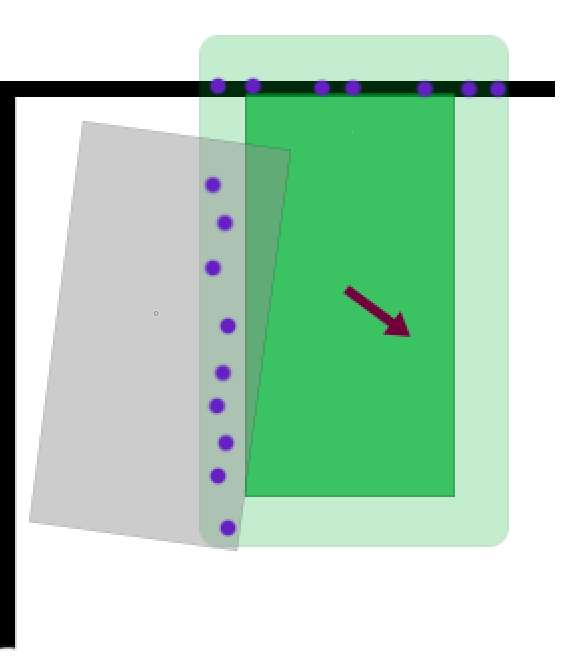
\includegraphics[height=1.2in]{Figures/step_1}
\begin{overpic}[height=1.2in]{Figures/push_3.png}%
\put(350,-100){(b)}%
\end{overpic}
\hspace{0.1in}
% 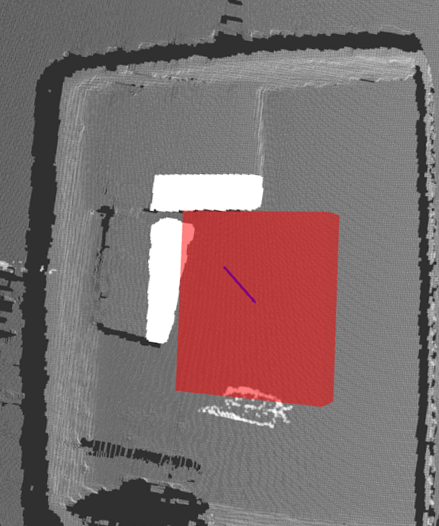
\includegraphics[height=1.2in]{Figures/push_3.png}
\begin{overpic}[height=1.2in]{Figures/tight_push_00.png}%
\put(450,-70){(c)}%
\end{overpic}
% 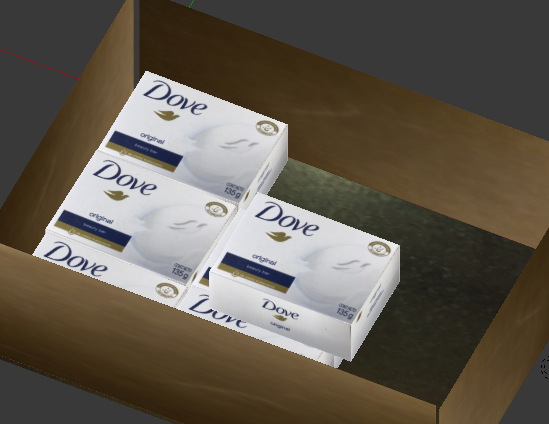
\includegraphics[height=1.2in]{Figures/tight_push_00.png}
\begin{overpic}[height=1.2in]{Figures/tight_push_02.png}%
\put(450,-70){(d)}%
\end{overpic}
% 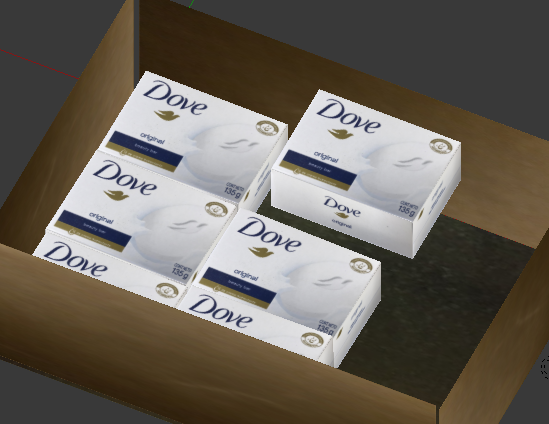
\includegraphics[height=1.2in]{Figures/tight_push_02.png}
\begin{overpic}[height=1.2in]{Figures/tight_push_03.png}%
\put(450,-70){(e)}%
\end{overpic}
% 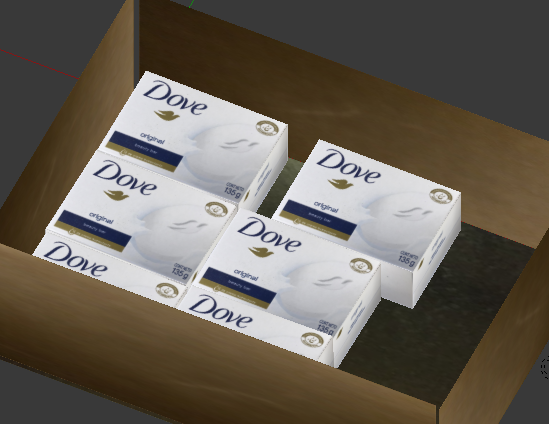
\includegraphics[height=1.2in]{Figures/tight_push_03.png}
% \vspace{-0.1in}
\caption{Adaptive pushing: (a) The black border is the bin and the gray rectangle a previously placed object. The green rectangle represents the target pose for the current object. The light green boundary represents an $\varepsilon$-expanded model that intersects the point cloud at the purple points. These points result in the black vector that pushes the object away from them. (b) A screen shot of a scene's point cloud, where the white points are collision points with previously placed objects and the red volume shows the computed pre-push pose for the new object.
Adaptive pushing in the boundary case (the sixth object). (c)The target object is moving at the upper level and from the pre-push pose to the boundary. (d) The target object is being pushed against the boundary and then pushed down to the bottom level. (e) The target object is moved towards its target pose at the bottom level.
}
\label{fig:adaptive-pushing}
% \vspace{-0.2in}
\end{figure*}



%In the problem of packing in a tight space, failures tend to arise due to the uncertainties from perception of the object and the environment. In order to increase the robustness of packing, we propose a novel manipulation primitive we call "Push-Place". This primitive takes advantage of the compliance of the objects and environments to robustly placing an object in a tight bin. The idea is that instead of directly placing the object to its target position, while still attaching the object to the end-effector, we will first move the object to an intermediate position, then push the object towards its target position. This method has two main benefits: first, in finding the intermediate position, we minimize the probability of collision between the object and the environment;second, during the course of pushing, in addition to moving the target object to its desired position, the interaction between objects will also correct the misalignment of previous packed objects.     

Directly placing objects at the goal pose $\hat{p}^i$ into bin $\btarget$ is prone to placement failures due to errors in perception as well as prior placements. This may result in damaging the objects. A safer alternative is to drop the object from a certain height, right above the goal pose, so as to avoid pressing against previously erroneously placed objects. Still, however, this alternative results in low quality packing. A key realization is that during placement, the object being manipulated will inevitably approach or even collide with other objects or the target container. To sidestep undesirable collisions, an {\em adaptive pushing} primitive is developed, which directly operates over point cloud data for the target bin. 


The process is detailed in algorithm~\ref{algo:PushPlace}. The adaptive pushing begins by growing the object model at the target pose $\hat{p}^i$. Given the uncertainty value $\varepsilon$, the model is enlarged by  $2\varepsilon$ along each dimension. The enlarged model is intersected with the point cloud to retrieve collision points. A collision vector is computed as a vector pointing from a collision point to the center of the object model. Summing all collision vectors yields the displacement vector. By iteratively moving the object model along the unit displacement vector, where the displacement vector is recomputed after each movement, a collision-free pre-push pose for the object is obtained. An example scene is shown in Fig.~\ref{fig:adaptive-pushing}. During the execution, the robot first moves the object above the pre-push pose, then lowers the object to the pre-push pose and finally pushes the object to the target pose. 

% The adaptive pushing primitive begins by moving the picked-up object to a pose with a larger $z$-value than the goal pose $\hat{p}^i$. It then tries to find a set of intermediate target poses for generating collision-free paths for the object and the end-effector as the object is gradually lowered to its final desired pose. The idea behind generating one such intermediate pose is shown in Fig.~\ref{fig:adaptive-pushing}, where a {\em displacement vector} is shown. At any point when a new intermediate pose is to be generated, to counter the potential negative effects caused by pose uncertainty, an $\varepsilon$-expanded model of the object's current estimated pose (i.e., growing the object model by $2\varepsilon$ along each dimension) is intersected with the point cloud. Based on the intersection, a displacement vector defining a new intermediate pose is  generated that guides the object away from potential collisions. 

%An intermediate pose is denoted a {\em pre-push pose}. Algorithm~\ref{algo:PushPlace} outlines the process of finding these pre-push poses. 

\begin{algorithm}
\small
\DontPrintSemicolon
\KwIn{Pointcloud $C$,  target pose $\pose_t$, bounding box size $S$}
\KwOut{Push direction $d$, pre-push pose $\pose_{pre}$  }
$\pose_{pre} \gets \pose_t$ \;
 $bbox \gets$ GenerateBoundingBox($\pose_{pre}, S$)  \;
\While{$bbox$ \normalfont is in collision}{
$C_{collision} \gets$ Intersection($bbox , C$) \;
 $u_{push} \gets$ GeneratePushVector($C_{collision}, \pose_{pre}$)\;
 $\pose_{pre} \gets \pose_{pre} + u_{push}$\;
 \lIf{\normalfont IsLocalMinimum($\pose_{pre}$)}{
    decrease $S$
 }
 $bbox \gets$ GenerateBoundingBox($\pose_{pre}, S$)
}
$d \gets \pose_t - \pose_{pre}$\;
\Return{$d, \pose_{pre}$}\;
\caption{{\sc PushPlace-Planner}}
\label{algo:PushPlace}
\end{algorithm}

\begin{algorithm}
\small
\DontPrintSemicolon
\KwIn{Pointcloud $C$,  target pose $\pose_t$, bounding box size $S$}
\KwOut{Push path $path$ }
$\pose_{higher} \gets \pose_{t}   $\;
$\pose_{higher}.z \gets \pose_{t}.z + obj\_height   $\;
$(d, \pose_{pre}) \gets$ PushPlace-Planner$($C$, \pose_{higher}, S)$  \;
$\pose_{wall} \gets$ ProjectPoseToWall($\pose_{higher})$   \;
$\pose_{down} \gets \pose_{wall}$  \;
$\pose_{down}.z \gets \pose_{wall}.z - obj\_height$   \;
$path \gets (\pose_{wall}, \pose_{pre})$   \;
$path \gets (\pose_{down}, \pose_{wall})$\;
$path   \gets (\pose_{t}, \pose_{down})$    \;
\Return{$path$}\; 
\caption{{\sc TightPushPlace-Planner}}
\label{algo:TightPushPlace}
\end{algorithm}


For special scenario where objects need to be packed tightly with no clearance, in order to place the objects near the boundary robustly, it requires additional steps in pushing. The process is detailed in algorithm~\ref{algo:TightPushPlace}. In this case, since there is no space for pushing in the same layer of the target pose, the target object will first be moved at the upper layer and use the boundary of the container to correct potential noise in the object pose. The compliance of the container boundary will also enable the object to fit the tight gap when the object is pushed down to target level. The process of placing one object to an boundary pose is illustrated in Fig.~\ref{fig:adaptive-pushing}. This procedure is required for each object that is at the boundary of the container. 

% \begin{figure}[t]
% \centering
% 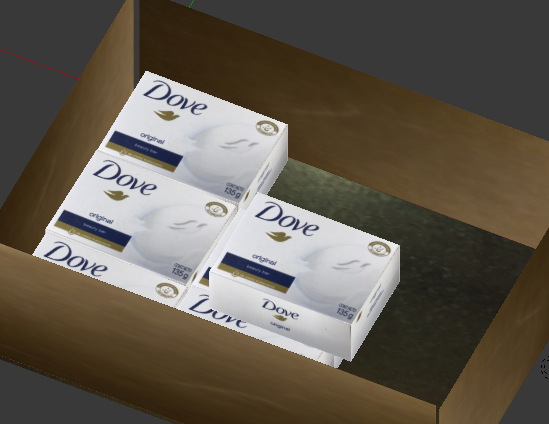
\includegraphics[width=0.15\textwidth]{Figures/tight_push_00.png}
% 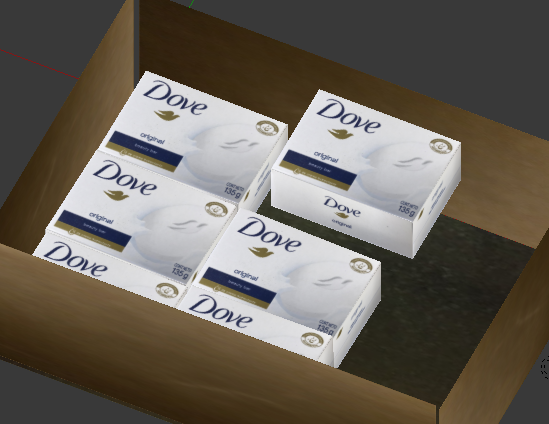
\includegraphics[width=0.15\textwidth]{Figures/tight_push_02.png}
% 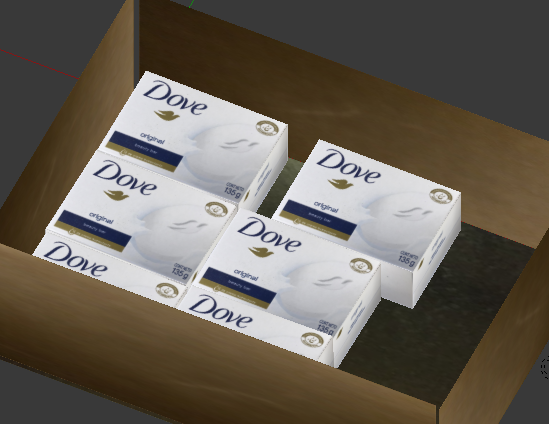
\includegraphics[width=0.15\textwidth]{Figures/tight_push_03.png}
% \vspace{-0.1in}
% \caption{Adaptive pushing in the boundary case (the sixth object). (left)The target object is moving at the upper level and from the pre-push pose to the boundary. (middle) The target object is being pushed against the boundary and then pushed down to the bottom level. (right) The target object is moved towards its target pose at the bottom level.}

% % A screen shot where the green volume is the ground truth pose for the object and the red one is where the object should be moved next.}
% %\label{fig:workspace}
% \label{fig:tight-pushing}
% \vspace{0.1in}
% \end{figure}

%Line 1-2 initialize the pre-push pose $\pose_{pre}$ and the bounding box $bbox$ generated at $\pose_{pre}$. The function GenerateBoundingBox generates a bounding box centered at the given pose with the given size. In line 2, the size $S$ is bigger than the actual size of the object to reflect the uncertainties of the estimated pose. Line 3-8 of the algorithm iteratively tries to find a collision-free pre-push pose. The strategy is to move the bounding box towards the direction that will decrease the collision region. In line 4, Function Intersection($bbox, C$) will calculate the intersection points between bounding box $bbox$ and the environment pointcloud $C$. $C_{collision}$ will be passed to function GeneratePushVector to generate a local unit vector to move the current pre-push pose. In function GeneratePushVector($C_{collision}, \pose_{pre}$), all the vectors from points of $C_{collision}$ to the pre-push pose $\pose_{pre}$ are normalized, the summation of all these unit vectors is returned as the local push vector $u_{push}$. Then $u_{push}$ is used to update the pre-push pose $\pose_{pre}$. At narrow region, this local optimization process can be stuck at local minimum. The strategy we used is to reduce the size $S$ for generating bounding box. In the experiments, this usually helped to find a valid pre-push pose.



%\subsection{Packing With Use Of Non-Prehensile Push}
\subsection{Fine Correction using Push and Pull Primitives}
%As a local optimization strategy, the dynamic pushing primitive does not provide %guaranteed success. In the semi-structured setup of this work, however, it %provides a significant boost to robustness. 

\begin{figure*}
\centering
\begin{tabular}{@{}c@{}c@{}}
%\cline{2-2}
& No corrective actions\\
\multirow{3}{*}{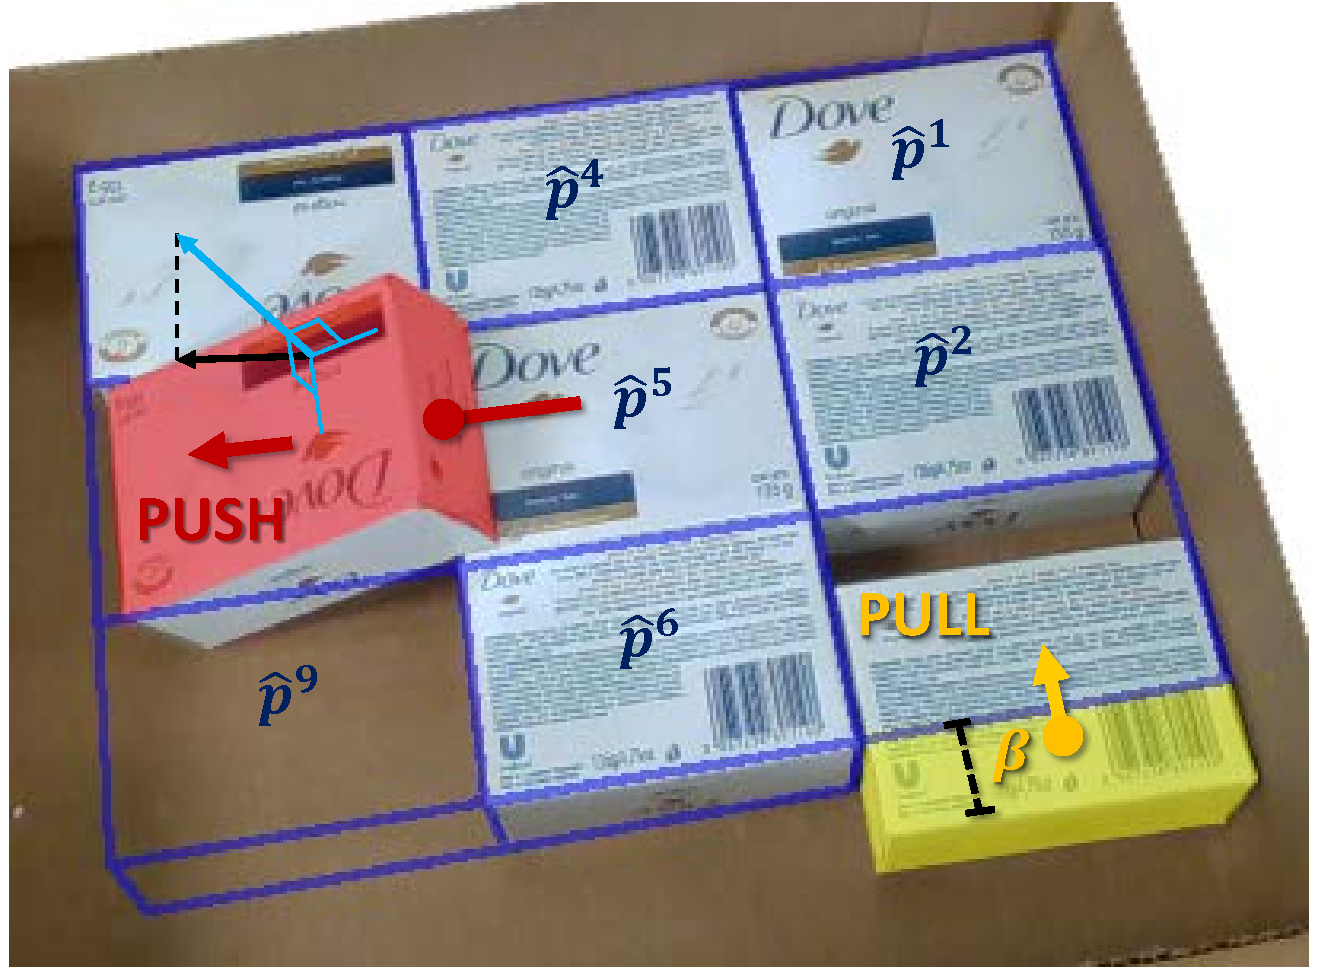
\includegraphics[width=0.24\textwidth]{Figures/finer_fix.pdf}}
& 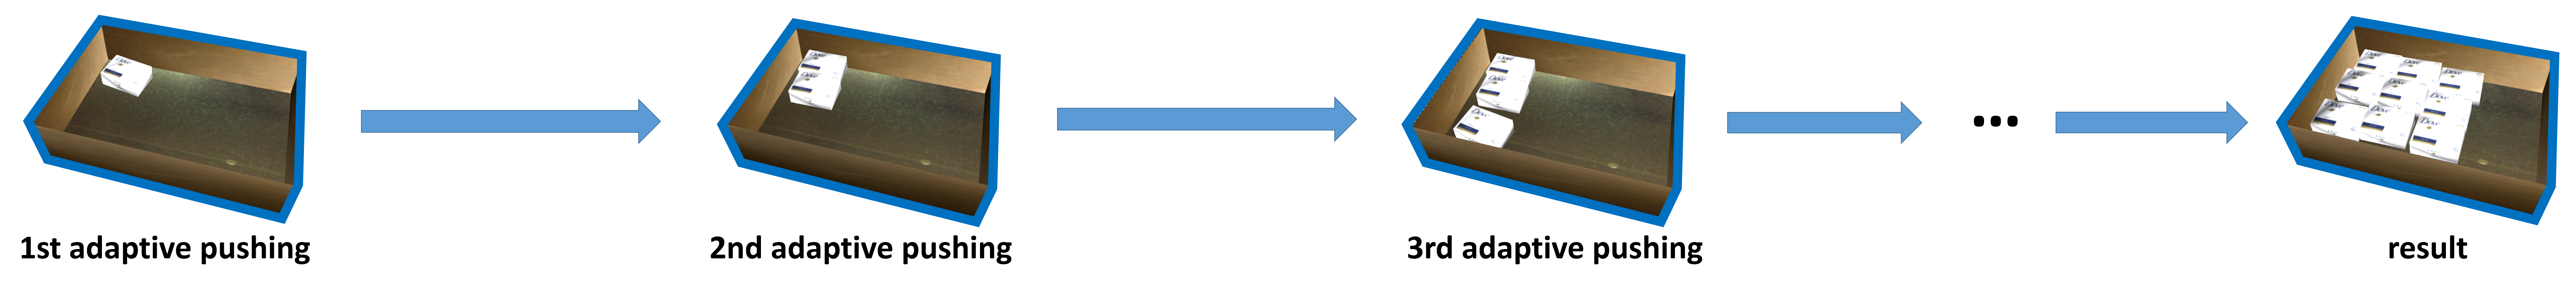
\includegraphics[width=0.75\textwidth,valign=t]{./Figures/res_step_adaptive.png}
\\\cline{2-2}
& Full pipeline\\
& 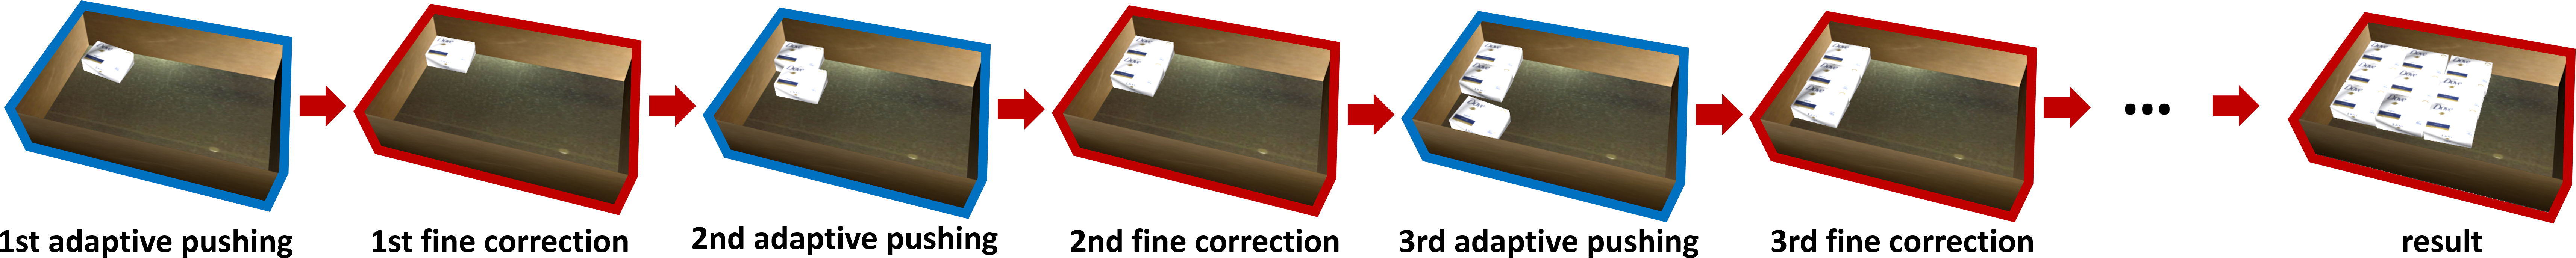
\includegraphics[width=0.75\textwidth]{./Figures/res_step_full.png}
\\%\cline{2-2}
\end{tabular}
\caption{Fine layout adjustment and correction.}
\label{fig:finer_fix}
\end{figure*}

The final primitive deals with the remaining failure cases. Fine corrections are required because objects can be placed in incorrect poses due to unexpected collisions as well as calibration and pose estimation errors.  The proposed corrective manipulation procedure continuously monitors the scene and triggers corrective actions whenever necessary. 

%Even small alignment errors can have a domino effect on the  packing task and make the placement of remaining objects infeasible. 

\begin{comment}
\begin{wrapfigure}{r}{1.5in}
\vspace{-.2in}
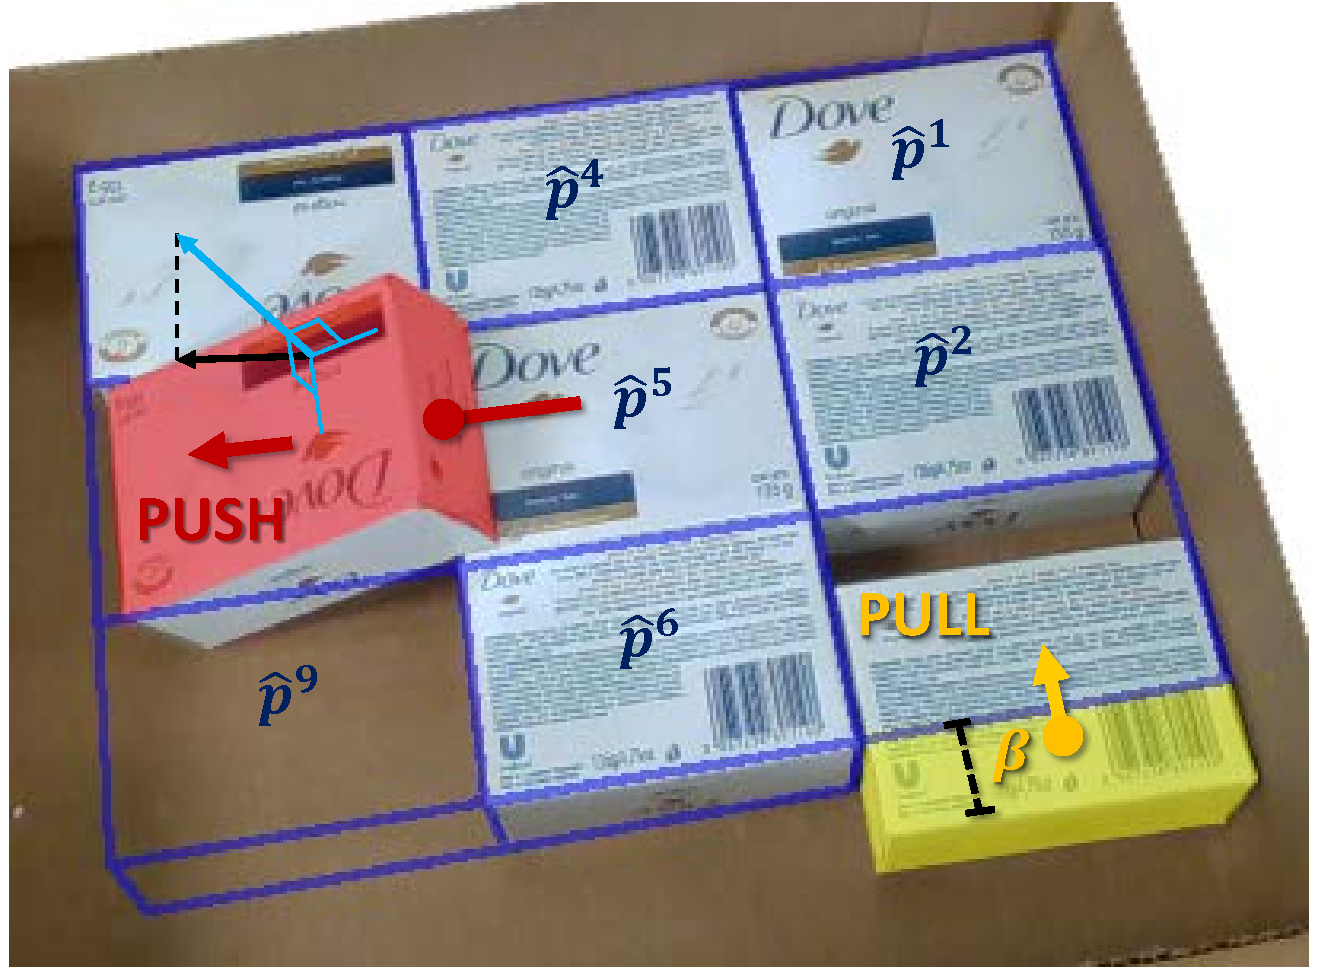
\includegraphics[width=1.49in]{Figures/finer_fix.pdf}
\vspace{-.3in}
\caption{Fine layout adjustment and correction.}
\label{fig:finer_fix}
\vspace{-.15in}
\end{wrapfigure}
\end{comment}

The process first removes the background, the box, the robot's arm and end-effector from the observed point cloud and computes its surface normals.
The observed point cloud is then compared against the desired alignment of the objects in their target poses. As shown in Fig.~\ref{fig:finer_fix}, two types of misalignment errors can occur. The first type occurs when the top surface normal of an object is not perpendicular to the support surface. This error is corrected by pushing the object along a direction and for a distance computed based on its surface normal in a manner that makes it aligned with the support surface. 
The second type of error happens when a peripheral object is not entirely within the desired footprint of the pile. The proposed procedure systematically detects pivot points that are outside the desired footprint of the pile and pulls their objects inside accordingly. The correction is repeated until the point cloud is  aligned with the desired goal poses given a threshold
%$\epsilon$
\changkyu{$\tau$}, or a timeout occurs.

\changkyu{
% [changkyu] uncommented 

Given the alignment pose $\hat{\pose}^i$ which defines the six \textit{facets} $\hat{F}^i = \{\hat{f}_1^i,\dots,\hat{f}_6^i\}$ of the cubic, the pre-processed observation $\mathcal{I}$ is split into disjoint sets $\{X^i\}_{i=0}^n$ where $X^i$ is the point cloud cropped by $\hat{F}^i$ and $X^0$ is the remaining.
Starting with the furthermost point cloud $X^i$ from a pivot point $x_{pivot}$, e.g. the upper right corner of the box, we determine if it agrees with $\atarget$ by measuring the distance between the point cloud $X^i$ and the closest facet $\hat{f}_j^{i'}$ that is not in parallel to the xy-plane as well as the normal difference.
Once a disagreement is detected, an appropriate pushing or pulling action is executed as described in Algorithm \ref{algo:FinerFix}.
For example, the objects leaning against other objects, which accompany a significant normal disagreement, will be pushed away to be slipped, and the objects translated from its desired position will be pulled towards it.
The correction is repeated until all the observation agree with $\atarget$ or timeout.

{\small
\begin{algorithm}
\KwIn{
	$\atarget = \{ \hat{p}^1, \ldots, \hat{p}^n \}$, an error threshold $\tau$, the point cloud segments $\{X[i]\}_{i=0}^{n}$, a corner point $x_{pivot}$
}
\Repeat{Timeout}
{
Sort centers of $X[i]$ based on increasing distance to $x_{pivot}$;\\

	\For{$i\leftarrow 0; i\leq n; i\leftarrow i+1$}
	{
		{\scriptsize\tcp{Check if X[i] is not horizontally placed}}
		\If{ $\{x | normal(x).z < 1 - \epsilon, x \in X[i]\} \neq \emptyset$ }
		{
        Push segment $X[i]$ from a side to translate its center $x_c$  with  $\alpha \times normal(x_c)$, after projecting vector $normal(x_c)$ to the XY plane, and where $\alpha$ is a small constant; \\
			break
		}
		{\scriptsize\tcp{Check if X[i] is horizontally off-set}}
        Let object\_box($\hat{p}^{i'}$) be the closest target to $X[i]$, and let $\beta$ be the {\it Frechet distance} between $X[i]$ and object\_box($\hat{p}^{i'}$).\\
%		\If{ $X[i]$ does not fit with $\hat{p}^i$ }
		{			
			\If{$\beta > \tau$}
			{
				Pull $X[i]$ toward $\hat{p}^{i'}$ with distance $\beta$;\\
				break
			}
		}
	}
	break
}
\caption{Realignment}
\label{algo:FinerFix}
\end{algorithm}
}

}

\begin{comment}
{\small
\begin{algorithm}
\KwIn{
	$\atarget = \{ \hat{p}^1, \ldots, \hat{p}^n \}$, an error threshold $\tau$
}
\Repeat{Timeout}
{
Get {\tt RGB-D} input $\mathcal{I}$;\\
\For{$i := 1; i \leq n; i\leftarrow i+1$}
{
	{\scriptsize\tcc{X[i]: point cloud segment for $o^i$}}
    $X[i] \leftarrow \mathcal{I} \cap \text{object\_box}(\hat{p}^i)$,
	$\mathcal{I} \leftarrow \mathcal{I} \backslash X[i]$
    
}
$X[0] = \mathcal{I}$;\\
$x_{pivot}$ is any corner point in the convex hull of $\mathcal{I}$;\\
Sort centers of $X[i]$ based on increasing distance to $x_{pivot}$;\\

	\For{$i\leftarrow 0; i\leq n; i\leftarrow i+1$}
	{
		{\scriptsize\tcc{Check if X[i] is not horizontally placed}}
		\If{ $\{x | normal(x).z < 1 - \epsilon, x \in X[i]\} \neq \emptyset$ }
		{
        Push segment $X[i]$ from a side to translate its center $x_c$  with  $\alpha \times normal(x_c)$, after projecting vector $normal(x_c)$ to the XY plane, and where $\alpha$ is a small constant; \\
			break
		}
		{\scriptsize\tcc{Check if X[i] is horizontally off-set}}
        Let object\_box($\hat{p}^{i'}$) be the closest target to $X[i]$, and let $\beta$ be the {\it Frechet distance} between $X[i]$ and object\_box($\hat{p}^{i'}$).\\
%		\If{ $X[i]$ does not fit with $\hat{p}^i$ }
		{			
			\If{$\beta > \tau$}
			{
				Pull $X[i]$ toward $\hat{p}^{i'}$ with distance $\beta$;\\
				break
			}
		}
	}
	break
}
\caption{Realignment}
\label{algo:FinerFix}
\end{algorithm}
}
\end{comment}